%%%%%%%%%%%%%%%%%%%%%%%%%%%%%%%%%%%%%%%%%%%%%%%%%%%%%%%%%%%%%%%%%%%%%%%%%%%%%%%
\chapter{More basics}

\begin{comment}
%%%%%%%%%%%%%%%%%%%%%%%%%%%%%%%%%%%%%%%%%%%%%%%%%%%%%%%%%%%%%%%%%%%%%%%%%%%%%%%
\section{Choice of $\log$ / Determination $\tilde\theta$ of $\theta$}
% \begin{figure}[!htbp] %{{{
%   \centering
%  \begin{subfigure}[b]{0.4\textwidth}
    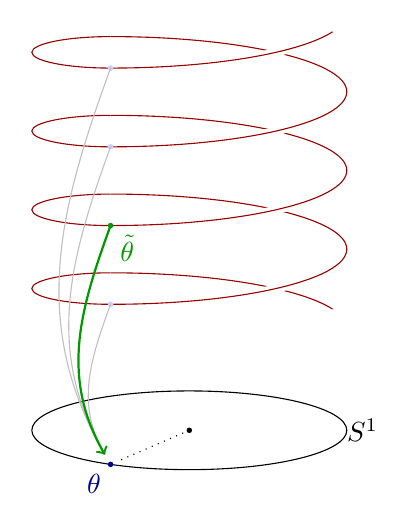
\begin{tikzpicture}[scale=1]
      \node[] (zero) at (0,0) {};
      \fill (zero) circle (1pt);
      \draw (0,-0.5) arc (270:-90:2 and 0.5);

      \node (theta) at ({cos(240) * 2},{sin(240) * 0.5}) {};
      % \node [below left of=theta,blue!40!white] {$\theta$};

      \draw[dotted] (0,0) -- (theta);
      \fill[blue!60!black] (theta) circle (1pt);


      \draw[red!60!black] (-1,2) arc (270:200:-3 and -0.7);
      \draw[line width=3pt,white] (-1,2) arc (270:90:1 and -0.2) arc (270:90:-3 and 0.7);
      \draw[red!60!black] (-1,2) arc (270:90:1 and -0.2) arc (270:90:-3 and 0.7);
      \fill[blue!20!white] (-1,1.6) circle (1pt);

      \draw[line width=3pt,white] (-1,3) arc (270:90:1 and -0.2) arc (270:90:-3 and 0.7);
      \draw[red!60!black] (-1,3) arc (270:90:1 and -0.2) arc (270:90:-3 and 0.7);
      \fill[green!60!black] (-1,2.6) circle (1pt);

      \draw[line width=3pt,white] (-1,4) arc (270:90:1 and -0.2) arc (270:90:-3 and 0.7);
      \draw[red!60!black] (-1,4) arc (270:90:1 and -0.2) arc (270:90:-3 and 0.7);
      \fill[blue!20!white] (-1,3.6) circle (1pt);

      \draw[line width=3pt,white] (-1,5) arc (270:90:1 and -0.2) arc (270:200:-3 and 0.7);
      \draw[red!60!black] (-1,5) arc (270:90:1 and -0.2) arc (270:200:-3 and 0.7);
      \fill[blue!20!white] (-1,4.6) circle (1pt);


      \draw[->,gray!50!white] (-1,1.6) to[out=250,in=120] (theta);
      \draw[->,gray!50!white] (-1,3.6) to[out=250,in=120] (theta);
      \draw[->,gray!50!white] (-1,4.6) to[out=250,in=120] (theta);
      \draw[->,green!60!black,thick] (-1,2.6) to[out=250,in=120] (theta);
      \node[below left,blue!60!black] at (theta) {$\theta$};
      \node[below right,green!60!black] at (-1,2.6) {$\tilde\theta$};

      \node[red!60!black] at (2.2,4.8) {$\R$};
      \node at (2.2,0) {$S^1$};
    \end{tikzpicture}
    % \caption{Universal cover}
    % \label{fig:univCover}
  % \end{subfigure}%
  % \qquad
  % \begin{subfigure}[b]{0.4\textwidth}
    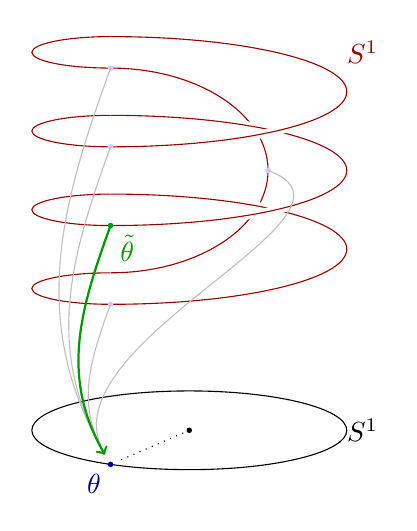
\begin{tikzpicture}[scale=1]
      \node[] (zero) at (0,0) {};
      \fill (zero) circle (1pt);
      \draw (0,-0.5) arc (270:-90:2 and 0.5);

      \node (theta) at ({cos(240) * 2},{sin(240) * 0.5}) {};
      % \node [below left of=theta,blue!40!white] {$\theta$};

      \draw[dotted] (0,0) -- (theta);
      \fill[blue!60!black] (theta) circle (1pt);


      \draw[line width=3pt,white] (-1,5) arc (270:90:1 and -0.2) arc (270:200:-3 and 0.7);
      \draw[red!60!black] (-1,5) arc (270:90:1 and -0.2) arc (270:90:-2 and -1.3);
      \fill[blue!20!white] (-1,4.6) circle (1pt);
      \fill[blue!20!white] (1,3.3) circle (1pt);

      % \draw[red!60!black] (-1,2) arc (270:200:-3 and -0.7);
      \draw[line width=3pt,white] (-1,2) arc (270:90:1 and -0.2) arc (270:90:-3 and 0.7);
      \draw[red!60!black] (-1,2) arc (270:90:1 and -0.2) arc (270:90:-3 and 0.7);
      \fill[blue!20!white] (-1,1.6) circle (1pt);

      \draw[line width=3pt,white] (-1,3) arc (270:90:1 and -0.2) arc (270:90:-3 and 0.7);
      \draw[red!60!black] (-1,3) arc (270:90:1 and -0.2) arc (270:90:-3 and 0.7);
      \fill[green!60!black] (-1,2.6) circle (1pt);

      \draw[line width=3pt,white] (-1,4) arc (270:90:1 and -0.2) arc (270:90:-3 and 0.7);
      \draw[red!60!black] (-1,4) arc (270:90:1 and -0.2) arc (270:90:-3 and 0.7);
      \fill[blue!20!white] (-1,3.6) circle (1pt);



      \draw[->,gray!50!white] (-1,1.6) to[out=250,in=120] (theta);
      \draw[->,gray!50!white] (-1,3.6) to[out=250,in=120] (theta);
      \draw[->,gray!50!white] (-1,4.6) to[out=250,in=120] (theta);
      \draw[->,gray!50!white] (1,3.3) to[out=-20,in=120] (theta);
      \draw[->,green!60!black,thick] (-1,2.6) to[out=250,in=120] (theta);
      \node[below left,blue!60!black] at (theta) {$\theta$};
      \node[below right,green!60!black] at (-1,2.6) {$\tilde\theta$};

      \node[red!60!black] at (2.2,4.8) {$S^1$};
      \node at (2.2,0) {$S^1$};
    \end{tikzpicture}
    % \caption{$q$-sheet cover}
    % \label{fig:qCover}
  % \end{subfigure}
  % \caption{Covers}\label{fig:covers}
% \end{figure} %}}}
\paragraph{Universal cover:}
\[
  \R\to S^1; \nu \mapsto e^{i\nu}
\]
\TODO{}

\paragraph{$q$-sheet cover:}
\[
  S^1\to S^1; \nu \mapsto \nu^q
\]
\TODO{}
\end{comment}

%%%%%%%%%%%%%%%%%%%%%%%%%%%%%%%%%%%%%%%%%%%%%%%%%%%%%%%%%%%%%%%%%%%%%%%%%%%%%%%
\section{Semidirect products}
\begin{comment}
  see
  \begin{itemize}
    \item \url{http://nlab.mathforge.org/nlab/show/semidirect+product+group}
    \item \url{http://en.wikipedia.org/wiki/Semidirect_product}
    \item \cite{Robinson2003An}
  \end{itemize}
\end{comment}
We will refer to \cite[75]{Robinson2003An} for semidirect products.
Let $G$ be a group with a normal subgroup $N$ ($N\vartriangleleft G$) and a
subgroup $H$ such that
\[
  G=NH\qquad\text{and}\qquad N\cap H=1.
\]
Then $G$ is said to be the \emph{(internal) semidirect product} of $N$ and $H$,
$G=N\rtimes H$.
\begin{rem}
  \begin{enumerate}
    \item Each element $g\in G$ has a unique decomposition $g=nh$ with $n\in N$
      and $h\in H$. Since
      \begin{itemize}
        \item[] for $g=n'h'$ another such expression, then
          $(n')^{-1}n=h'h^{-1}\in N\cap H=1$ such that $n=n'$ and $h=h'$.
      \end{itemize}
    \item Conjugation in $N$ by an element $h\in H$ defines an automorphism of
      $N$, say $\rho(h)$ which satisfies for $h_i\in H$
      \[
        \rho(h_1,h_2)=\rho(h_1)\rho(h_2)
      \]
      and thus $\rho:H\to\Aut(N)$ is a homomorphism.
  \end{enumerate}
\end{rem}
In the other direction, one can get from $N$, $H$ and a given homomorphism
$\rho:H\to\Aut(N)$ the same structure back. This will be the so-called
\emph{external semidirect product}. It is defined by the underlying group
\[
  G:=\left\{(n,h)\mid n\in N,h\in H\right\}
\]
together with the multiplication
\begin{align*}
  G\times G&\to G
\\\left((n_1,h_1),(n_2,h_2)\right)&\mapsto(n_1\rho(h_1)(n_2),h_1h_2)
\end{align*}
with the identity element $(1_N,1_H)$ and the inverse of $(n,h)$ given by
$(\rho(h^{-1})(n^-1),h^-1)$. In $G$ there are the natural subgroups
\[
  \bar N=\{(n,1_H)\mid n\in N)\}
  \qquad\text{and}\qquad
  \bar H=\{(1_N,h)\mid h\in H)\}
\]
which are canonically isomorphic to $N$ and $H$ respectively. For $n\in N$ and
$h\in H$ we have
\[
  (n,1_H)(1_N,h)=(n\underset{\id_N}{\underbrace{\rho(1_H)}}(1_N),h)
  =(n,h)\in \bar N\bar H \,.
\]
It follows that $G=\bar N\bar H$ and $\bar N\cap\bar H=1$. To check that
$G=\bar N\rtimes\bar H$ we only have to show that $\bar N$ is normal in $G$.
Let $n,n'\in N$ and $h\in H$ then
\begin{align*}
  (n,h)(n',1_H)(n,h)^{-1}
  &=(n,h)(n',1_H)(\rho(h^{-1})(n^{-1}),h^{-1})
  \\&=(n\rho(h)(n'),h)(\rho(h^{-1})(n^{-1}),h^{-1})
  \\&=(n\rho(h)(n')\rho(h)\rho(h^{-1})(n^{-1}),1_H)
  \\&=(n\rho(h)(n')n^{-1},1_H) \in \bar N \,.
\end{align*}

In the case, where $\rho$ is the trivial homomorphism
\begin{align*}
  \rho:H&\to\Aut(N)
\\h&\mapsto \id_N
\end{align*}
the elements of $\bar N$ and $\bar H$ commute, so that $G$ becomes the direct
product $N\times H$. Thus the semidirect product is a generalization of the
direct product of two groups.

\TODO[from splitting exact sequence]

%%%%%%%%%%%%%%%%%%%%%%%%%%%%%%%%%%%%%%%%%%%%%%%%%%%%%%%%%%%%%%%%%%%%%%%%%%%%%%%
\section{Faithful representations} \label{sec:faithRepre}
\PROBLEM[Passt das hier?]
\cite[Def.4.1]{hall2003lie} says the following about faithful representations:
\begin{defn}
  \begin{comment}
    See:
    \begin{itemize}
      \item \cite[Def.4.1]{hall2003lie}
      \item \url{http://nlab.mathforge.org/nlab/show/faithful+representation}
    \end{itemize}
  \end{comment}
  Let $G$ be a matrix\PROBLEM{} Lie group. Then a \emph{(finite-dimensional
  complex) representation} of $G$ is a Lie group homomorphism
  \[
    \rho:G\to\Gl(V)
  \]
  where
  \begin{itemize}
    \item $V$ is a finite-dimensional complex vector space.
  \end{itemize}
  If $\rho$ is a one-to-one homomorphism, then the representation is called
  \emph{faithful}.
  \begin{comment}
    \textbf{Other criterion:}
    If the associated homomorphism $G\to\Aut(V)$ is injective, then the
    representation is \emph{faithful}.
  \end{comment}
  \begin{s-rem}
    If a representation $\rho$ is a faithful representation of a matrix Lie
    group $G$ then $\{\rho(A)\mid A\in G\}$ is a group of matrices that is
    isomorphic to the original group $G$. Thus, $\rho$ allows us to represent
    $G$ as a group of matrices.
  \end{s-rem}
\end{defn}

%%%%%%%%%%%%%%%%%%%%%%%%%%%%%%%%%%%%%%%%%%%%%%%%%%%%%%%%%%%%%%%%%%%%%%%%%%%%%%%
\chapter{Multisummability}\label{app:multisummability}
\begin{comment}
  \cite[Sec.III.2]{Loday1994},
  \cite[Chap.6]{Loday2014} and
  \cite[Chap.8]{Loday2014}
\end{comment}
\marginnote{\cite[111]{Loday2014}}
The aim of a theory of summation is  to associate with any series an asymptotic
function uniquely determined in a way as much natural as possible.
\rewrite{We will take this as a black box and only use the fact, that it makes
the asymptotic expansion unique.}
A useful and extensive resource for this topic is Loday-Richaud's
book~\cite{Loday2014}.

Let $[A^0]$ be a normal form and $\hat F\in\hat G(A^0)$ a formal
transformation and denote the transformed system by $A={}^{\hat F}\!A^0$.
\marginnote{\cite[Sec.III.2.1]{Loday1994}}
Let $\dot\phi=(\dot\phi_j)_{j\in J}\in\Gamma(\dot{\mathcal{V}};\Lambda(A^0))$
be a $1$-cocycle in the image of the equivalence class of $\hat F$ by $\exp$.

The following Proposition can be found in \cite[Prop.III.2.1]{Loday1994},
\cite[Thm.4.3.13]{Loday2014} and \cite[Thm.1]{BJL1979Birkhoff}.
\begin{prop}\label{prop:multisummability}
  There exists a \textbf{unique} family of realizations $(F_j)_{j\in J}$ of
  $\hat F$ over $\mathcal{V}$, i.e.\ matrices $F_j$ which are analytic on
  $V_j$, satisfy $[A^0,A]$ and are asymptotic to $\hat F$ on $V_j$, such that
  \[
    \dot\phi_j=F_{j-1}F_j^{-1}
  \]
  for every $j\in J$.
\end{prop}
When $\mathcal{V}$ is the, in section~\ref{sec:proofOfMatrixThm} defined,
cyclic covering $\cU^{\leq k_r}=:\cU$ and $\dot\phi$ is in its Stokes
form\TODO[~(cf.~??)], we call the realizations $F_{\alpha}$, the
\emph{sums of $\hat F$}.
\begin{defn}\label{defn:sumsLeftRight}
  \marginnote{\cite[Defn.III.2.2]{Loday1994}}
  Denote by $\alpha^+$ the next anti-Stokes direction on the right of $\alpha$
  we can define
  \begin{itemize}
    \item $S_\alpha^-(\hat F):=F_\alpha$ as the \emph{sum of $\hat F$ on the
      left of $\alpha$} and
    \item $S_\alpha^+(\hat F):=F_{\alpha^+}$ as the \emph{sum of $\hat F$ on
      the right of $\alpha$}.
  \end{itemize}
\end{defn}

\marginnote{\cite[883]{Loday1994}}
Let $\hat F_0\in\hat G(A^0)$ and $A^1={}^{\hat F_0}\!A^0$ and let
\[
  \exp_{A^1}(\hat F):G\backslash\hat G(A^1) \to H^1(S^1;\Lambda(A^1))
\]
be the Malgrange-Sibuya isomorphism (cf.\ Remark~\ref{rem:expNonNormalForm}).

The definition of the subsheaf $\Lambda^{\geq k}(A^1)$ of $\Lambda(A^1)$
\rewrite{needs a few additional justifications} (cf.\ \cite[883]{Loday1994}).
\begin{defn}
  \marginnote{\cite[Defn.III.2.3]{Loday1994}}
  A $1$-cocycle $\dot\phi=(\dot\phi_j)_{j\in J}$ is \emph{$k$-summable} if, for
  all $j\in J$, it satisfies the conditions
  \begin{enumerate}
    \item $\dot\phi_j$ is of level $\geq k$,
      i.e.\ $\phi_j\in\Gamma(\dot V_j;\Lambda^{\geq k}(A^1))$ and
    \item the opening of $\dot V_j$ is $\frac{\pi}{k}$.
  \end{enumerate}
  An element of $\hat F\in\hat G(A^1)$ is \emph{$k$-summable} when
  $\exp_{A^1}(\hat F)$ contains a $k$-summable cocycle.
\end{defn}

\marginnote{\cite[883]{Loday1994}}
If in a cohomology class is a $k$-summable cocycle, it is unique up to extra
trivial components.
The realizations of such a $k$-summable cocycle define the $k$-sums of
$\hat F$\comm{~in an essentially unique way}.
When $[A^1]$ is meromorphically equivalent to $[A^0]$,
i.e.\ $\hat F\in G(\!\{t\}\!)$, then
\begin{einr}
  $\hat F$ is $k$-summable
\end{einr}
if and only if
\begin{einr}
  its Stokes cocycle $\dot\phi=(\dot\phi_\alpha)_{\alpha\in\A}$ belongs to
  $\Gamma(\dot\cU^k;\Lambda^k)$.
\end{einr}
This occurs when the Stokes cocycle $\dot\phi$ of $\hat F$ bears only the level
$k$.

\begin{comment}
  \cite[883]{Loday1994} Turrittin's problem
\end{comment}

\begin{defn}\label{defn:singlDir}
  \marginnote{\cite[Defn.III.2.4]{Loday1994}}
  Let $\hat F\in\hat G(A^1)$ be $k$-summable and $(\dot\phi_j)_{j\in
  J}\in\prod_{j\in J}\Gamma(\dot V_j;\Lambda(A^1))$ the corresponding
  $k$-summable cocycle in $\exp_{A^1}(\hat F)$.

  To each $j\in J$ with a nontrivial $\dot\phi_j$ we define the bisecting
  direction of $\dot V_j$ as a \emph{singular direction for $\hat F$}.
\end{defn}

%%%%%%%%%%%%%%%%%%%%%%%%%%%%%%%%%%%%%%%%%%%%%%%%%%%%%%%%%%%%%%%%%%%%%%%%%%%%%%%
\section{Factorization}

Let $\dot f\in\Gamma(\dot\cU;\Lambda(A^0))$ be the Stokes cocycle associated to
$\hat F$ and $k=\max(\cK(\dot f))$ be the maximal level beared by $\dot f$.
We then know, since $\dot f^{\leq k}=\dot f$ and we have
corollary~\ref{cor:factorStokesGerms} that there is a unique decomposition
\[
  \dot f=\dot f^{<k}\dot g^k
  \qquad\text{and}\qquad
  \dot f=\dot f^k\dot f^{<k}
\]
where $\dot f^k$, $\dot g^k\in\Gamma(\dot\cU^{\leq k};\Lambda^k(A^0))$ and
$\dot f^{<k}\in\Gamma(\dot\cU^{\leq k};\Lambda^{<k}(A^0))$.

Since the cohomology class of $\dot f^{<k}$ belongs to $H^1(S^1;\Lambda(A^0))$
we know from the Malgrange-Sibuya theorem that there exists an, up to left
meromorphic factor unique, element $\hat F^{<0}$ of $\hat G(A^0)$ such that
$\dot f^{<k}$ belongs to $\exp_{A^0}(\hat F^{<k})$.

The Proposition \cite[Prop.III.2.6]{Loday1994} states the following.
\begin{prop}\label{prop:Lod.III.2.6}
  We have, that
  \begin{enumerate}
    \item $\hat F^k$ is $k$-summable with singular directions
      (cf.\ Definition~\ref{defn:singlDir}) belonging to
      $\A^k$
    \item The levels in the Stokes cocycle of $\hat F^{<k}$ are $<k$.
    \item The decomposition $\hat F=\hat F^{k}\hat F^{<k}$ with properties 1.\
      and 2.\ is essentially unique, that means:
      \begin{einr}
        if $\hat F=\hat H^k\hat H^{<k}$ is another decomposition, there is a
        matrix $h\in G(\!\{t\}\!)$ such that $\hat H^{<k}=h\hat F^{<k}$ and
        $\hat H^{k}=\hat F^{k}h^{-1}$.
      \end{einr}
  \end{enumerate}
\end{prop}
\begin{comment}
  \begin{proof}
    The first property \PROBLEM

    The property 2.\ is clear, \rewrite{since larger levels would require more
    singular directions}.

    The property 3.\ results from the fact that we must have
    \[
      \exp_{A^0}(\hat H^{<k})=\exp_{A^0}(\hat F^{<k}).
    \]
  \end{proof}
\end{comment}
We can use the Proposition~\ref{prop:Lod.III.2.6} to obtain the following
factorization on transformations, which can be found an Loday's
Paper~\cite[Thm.III.2.5]{Loday1994} or as~\cite[Thm.4.7]{Martinet1991}.
\begin{thm}\label{thm:summaFaktori}
  Let $\hat F\in\hat G(A^0)$ be a formal transformation and
  $\cK=\{k_1<k_2<\cdots<k_r\}$ be the set of levels of $[A^0]$. Then $\hat F$
  can be factored in
  \[
    \hat F=\hat F_r\hat F_{r-1}\dots\hat F_2\hat F_1
  \]
  where the matrices $\hat F_j$ are
  \begin{itemize}
    \item $k_j$-summable and
    \item with singular directions belonging to the set $\cA^{k_j}$.
  \end{itemize}
\end{thm}

\begin{comment}
  \begin{cor}
    \marginnote{\cite[Cor.III.2.7]{Loday1994}}
    Write the twisted cocycle $\dot\phi\in\exp_{A^1}(\hat F^k)$ in terms of
    sums of $\hat F^k$ over $\cU^{\leq k}$:
    \[
      \dot \phi_\alpha=S_\alpha^-(\hat F^k)^{-1}S_\alpha^+(\hat F^k)
      \text{, }
      \alpha\in\A^{\leq k} \,.
    \]
    Then, the factors $\dot g^k=(\dot g^k_\alpha)_{\alpha\in\A^{\leq k}}$ and
    $\dot f^k=(\dot f^k_\alpha)_{\alpha\in\A^{\leq k}}$ in the induced
    decompositions satisfy
    \begin{align*}
      \dot g_\alpha^k &=S_\alpha^+(\hat F^{<k})^{-1}
                        S_\alpha^-(\hat F^k)^{-1}
                        S_\alpha^+(\hat F^k)
                        S_\alpha^+(\hat F^{<k}) \,,
    \\\dot f_\alpha^k &=S_\alpha^-(\hat F^{<k})^{-1}
                        S_\alpha^-(\hat F^k)^{-1}
                        S_\alpha^+(\hat F^k)
                        S_\alpha^+(\hat F^{<k}) \,.
    \end{align*}
  \end{cor}
\end{comment}

\section{The map
  $g:G\backslash\hat G(A^0)\to\prod_{\alpha\in\cA}\Sto_\alpha(A^0)$}
  \label{sect:multisummmap}
There are other definitions, which are equivalent to
definition~\ref{defn:sumsLeftRight}. Since some of them are more direct
and do not use the $1$-cocycle, to which they correspond, they can be used to
obtain the corresponding $1$-cocycle. \rewrite{Many different approaches to
define the sums can be found in} \cite{Loday2014}.

Let us fix an ambassador $\hat F$ in $G\backslash\hat G(A^0)$. We then use
proposition~\ref{prop:multisummability} to obtain an $1$-cocycle.
\marginnote{\cite[Thm.4.3.13]{Loday2014}}
An element in $\prod_{\alpha\in\A}\Sto_\alpha(A^0)$ corresponding to $\hat F$
is found as
\[
  (\phi_{\alpha_1},\dots,\phi_{\alpha_\nu})
  \in\prod_{\alpha\in\A}\Sto_\alpha(A^0)
\]
by setting $\phi_\alpha:=
\left(S^-_\alpha(\hat F)\right)̂^{̀-1}S^+_\alpha(\hat F)\in\Sto_\alpha(A^0)$
(cf.\ Definition~\ref{defn:sumsLeftRight}).
\begin{rem}
  \marginnote{\cite[Defn.3.6]{boalch}}
  $S^+_\alpha(\hat F)t^Le^{Q(t^{-1})}$ is a solution of $[A]$ on the
  corresponding sector.
  \TODO[ or $S^-_\alpha(\hat F)t^Le^{Q(t^{-1})}$?  or
    $t^Le^{Q(t^{-1})}S^+_\alpha(\hat F)$?  or
  $t^Le^{Q(t^{-1})}S^-_\alpha(\hat F)$?]
  Using the equation (\ref{eq:representation}) we can write
  \[
    S^+_\alpha(\hat F)
    \cY_{0,\alpha}(t)
    =
    S^-_\alpha(\hat F)
    \cY_{0,\alpha}(t)C_{\cY_{0,\alpha}}
  \]
  thus the Stokes matrix $C_{\cY_{0,\alpha}}$ is a matrix, which
  describes the \rewrite{blending} between the two adjacent sectors.
  \TODO[see Loday's remarks on thm.4.3.13 in \cite{Loday2014}]
\end{rem}
\begin{comment}
  \begin{rem}
    For each $\alpha\in\A$ is $\phi_\alpha$
    \begin{enumerate}
      \item flat, since $\hat\phi_\alpha
           =\hat{\left(F_\alpha^+\right)̂^{̀-1}}\hat{F_\alpha^-}
           =\hat{F}^{̀-1}\hat{F}=\id$
      \item an isotropy, since
          ${}^{\phi_\alpha}\!A^0
           = {}^{\left(F_\alpha^+\right)̂^{̀-1}F_\alpha^-}\!A^0
           = {}^{\left(F_\alpha^+\right)̂^{̀-1}}\!\left({}^{F_\alpha^-}\!A^0\right)
           \overset{\PROBLEM{}}{=}{}^{\left(F_\alpha^+\right)̂^{̀-1}}\!A^1
           \overset{\PROBLEM{}}{=}A^0$
        % \begin{commentOUT}
        %   \begin{align*}
        %     {}^{\phi_\alpha}\!A^0
        %     &= (d\phi_\alpha)\phi_\alpha^{-1}+\phi_\alpha A^0
        %     \phi_\alpha^{-1}
        %   \\&=\left(
        %       d\left(\left(F_\alpha^+\right)̂^{̀-1}\right)̂F_\alpha^-
        %       +\left(F_\alpha^+\right)̂^{̀-1}dF_\alpha^-
        %     \right)\phi_\alpha^{-1}+\phi_\alpha A^0\phi_\alpha^{-1}
        %   \\&=\left(
        %       d\left(\left(F_\alpha^+\right)̂^{̀-1}\right)̂F_\alpha^-
        %       +\left(F_\alpha^+\right)̂^{̀-1}dF_\alpha^-
        %     \right) \left(F_\alpha^-\right)̂^{̀-1}F_\alpha^+
        %     +\left(F_\alpha^+\right)̂^{̀-1}F_\alpha^- A^0
        %      \left(F_\alpha^-\right)̂^{̀-1}F_\alpha^+
        %   \\&=
        %      d\left(\left(F_\alpha^+\right)̂^{̀-1}\right)̂F_\alpha^+
        %      +\left(F_\alpha^+\right)̂^{̀-1}dF_\alpha^-
        %      \left(F_\alpha^-\right)̂^{̀-1}F_\alpha^+
        %      +\left(F_\alpha^+\right)̂^{̀-1}F_\alpha^- A^0
        %      \left(F_\alpha^-\right)̂^{̀-1}F_\alpha^+
        %   \\&=\PROBLEM{}
        %   \\&=A^0
        %   \end{align*}
        % \end{commentOUT}
      \item of maximal decay, since \PROBLEM{}
    \end{enumerate}
  \end{rem}
\end{comment}
